\documentclass[10pt]{article}
\usepackage[utf8]{inputenc}
\usepackage[T1]{fontenc}
\usepackage{amsmath}
\usepackage{amsfonts}
\usepackage{amssymb}
\usepackage[version=4]{mhchem}
\usepackage{stmaryrd}
\usepackage{graphicx}
\usepackage[export]{adjustbox}
\graphicspath{ {./images/} }
\usepackage{caption}
\usepackage{hyperref}
\hypersetup{colorlinks=true, linkcolor=blue, filecolor=magenta, urlcolor=cyan,}
\urlstyle{same}

\begin{document}
\captionsetup{singlelinecheck=false}
\section*{Sample Exam Questions}
To elicit evidence of student achievement of the course learning objectives, exam questions assess both the application of the computational thinking practices and an understanding of the big ideas. Exam questions may assess achievement of multiple learning objectives. They may also address content from more than one essential knowledge statement. Exam questions may be accompanied by nontextual stimulus material such as diagrams, charts, or other graphical illustrations. The sample questions that follow illustrate the relationship between the curriculum framework and the AP Computer Science Principles Exam and serve as examples of the types of questions that will appear on the exam. Each question is accompanied by a table containing the enduring understandings, learning objectives, computational thinking practices, and essential knowledge statements that the question addresses. Note that in cases where multiple learning objectives are provided for a question, the primary learning objective is listed first, along with the associated computational thinking practice and essential knowledge statement(s).

\begin{enumerate}
  \item A video-streaming Web site uses 32 -bit integers to count the number of times each video has been played. In anticipation of some videos being played more times than can be represented with 32 bits, the Web site is planning to change to 64 -bit integers for the counter. Which of the following best describes the result of using 64 -bit integers instead of 32 -bit integers?\\
(A) 2 times as many values can be represented.\\
(B) 32 times as many values can be represented.\\
(C) $2^{32}$ times as many values can be represented.\\
(D) $32^{2}$ times as many values can be represented.
\end{enumerate}

\begin{center}
\begin{tabular}{|l|l|l|l|}
\hline
Enduring Understandings & Learning Objectives & Computational Thinking Practices & Essential Knowledge \\
\hline
2.1 A variety of abstractions built upon binary sequences can be used to represent all digital data. & 2.1.1 Describe the variety of abstractions used to represent data. [P3] & P3 Abstracting & \begin{tabular}{l}
2.1.1A \\
2.1.1B \\
2.1.1E \\
\end{tabular} \\
\hline
\end{tabular}
\end{center}

\begin{enumerate}
  \setcounter{enumi}{1}
  \item A programmer completes the user manual for a video game she has developed and realizes she has reversed the roles of goats and sheep throughout the text. Consider the programmer's goal of changing all occurrences of "goats" to "sheep" and all occurrences of "sheep" to "goats." The programmer will use the fact that the word "foxes" does not appear anywhere in the original text.
\end{enumerate}

Which of the following algorithms can be used to accomplish the programmer's goal?\\
(A) First, change all occurrences of "goats" to "sheep."

Then, change all occurrences of "sheep" to "goats."\\
(B) First, change all occurrences of "goats" to "sheep."

Then, change all occurrences of "sheep" to "goats."\\
Last, change all occurrences of "foxes" to "sheep."\\
(C) First, change all occurrences of "goats" to "foxes."

Then, change all occurrences of "sheep" to "goats."\\
Last, change all occurrences of "foxes" to "sheep."\\
(D) First, change all occurrences of "goats" to "foxes."

Then, change all occurrences of "foxes" to "sheep."\\
Last, change all occurrences of "sheep" to "goats."

\begin{center}
\begin{tabular}{|l|l|l|l|}
\hline
Enduring Understandings & Learning Objectives & Computational Thinking Practices & Essential Knowledge \\
\hline
4.1 Algorithms are precise sequences of instructions for processes that can be executed by a computer and are implemented using programming languages. & 4.1.1 Develop an algorithm for implementation in a program. [P2] & P2 Creating computational artifacts & \begin{tabular}{l}
4.1.1A \\
4.1.1B \\
\end{tabular} \\
\hline
\end{tabular}
\end{center}

\begin{enumerate}
  \setcounter{enumi}{2}
  \item ASCII is a character-encoding scheme that uses a numeric value to represent each character. For example, the uppercase letter "G" is represented by the decimal (base 10) value 71. A partial list of characters and their corresponding ASCII values are shown in the table below.
\end{enumerate}

\begin{center}
\begin{tabular}{|c|c|}
\hline
Decimal & ASCII Character \\
\hline
65 & A \\
\hline
66 & B \\
\hline
67 & C \\
\hline
68 & D \\
\hline
69 & E \\
\hline
70 & F \\
\hline
71 & G \\
\hline
72 & H \\
\hline
73 & I \\
\hline
74 & J \\
\hline
75 & K \\
\hline
76 & L \\
\hline
77 & M \\
\hline
\end{tabular}
\end{center}

\begin{center}
\begin{tabular}{|c|c|}
\hline
Decimal & ASCII Character \\
\hline
78 & N \\
\hline
79 & O \\
\hline
80 & P \\
\hline
81 & Q \\
\hline
82 & R \\
\hline
83 & S \\
\hline
84 & T \\
\hline
85 & U \\
\hline
86 & V \\
\hline
87 & W \\
\hline
88 & X \\
\hline
89 & Y \\
\hline
90 & Z \\
\hline
\end{tabular}
\end{center}

ASCII characters can also be represented by hexadecimal numbers. According to ASCII character encoding, which of the following letters is represented by the hexadecimal (base 16) number 56?\\
(A) A\\
(B) L\\
(C) V\\
(D) Y

\begin{center}
\begin{tabular}{|l|l|l|l|}
\hline
Enduring Understandings & Learning Objectives & Computational Thinking Practices & Essential Knowledge \\
\hline
2.1 A variety of abstractions built upon binary sequences can be used to represent all digital data. & 2.1.1 Describe the variety of abstractions used to represent data. [P3] & P3 Abstracting & \begin{tabular}{l}
2.1.1A \\
2.1.1C \\
2.1.1D \\
2.1.1E \\
2.1.1G \\
\end{tabular} \\
\hline
\end{tabular}
\end{center}

\begin{enumerate}
  \setcounter{enumi}{3}
  \item The figure below shows a circuit composed of two logic gates. The output of the circuit is true.\\
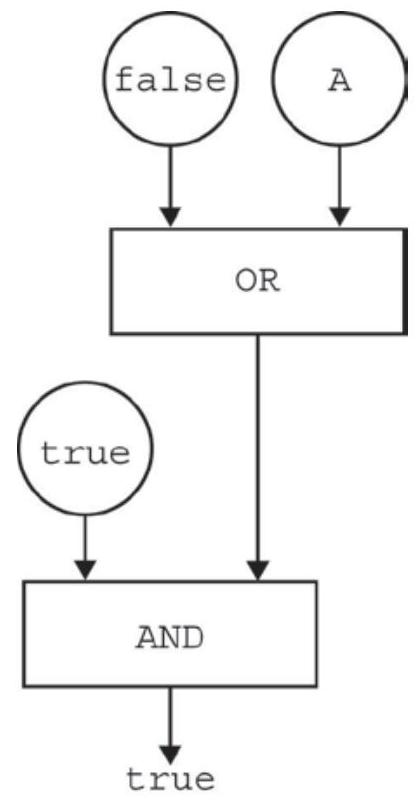
\includegraphics[max width=\textwidth, alt={}, center]{68b75e92-b243-4d72-a2a7-db8b0e1b4bf4-04_802_418_380_850}
\end{enumerate}

Which of the following is a true statement about input A?\\
(A) Input A must be true.\\
(B) Input A must be false.\\
(C) Input A can be either true or false.\\
(D) There is no possible value of input $A$ that will cause the circuit to have the output true.

\begin{center}
\begin{tabular}{|l|l|l|l|}
\hline
Enduring Understandings & Learning Objectives & Computational Thinking Practices & Essential Knowledge \\
\hline
2.2 Multiple levels of abstraction are used to write programs or to create other computational artifacts. & 2.2.3 Identify multiple levels of abstractions being used when writing programs. [P3] & P3 Abstracting & \begin{tabular}{l}
2.2.3E \\
2.2.3F \\
\end{tabular} \\
\hline
\end{tabular}
\end{center}

\begin{enumerate}
  \setcounter{enumi}{4}
  \item The following question uses a robot in a grid of squares. The robot is represented as a triangle, which is initially in the bottom left square of the grid and facing right.\\
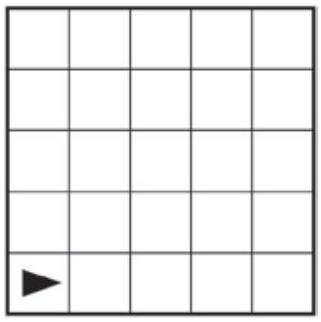
\includegraphics[max width=\textwidth, alt={}, center]{68b75e92-b243-4d72-a2a7-db8b0e1b4bf4-05_322_321_433_902}
\end{enumerate}

Consider the following code segment, which moves the robot in the grid.\\
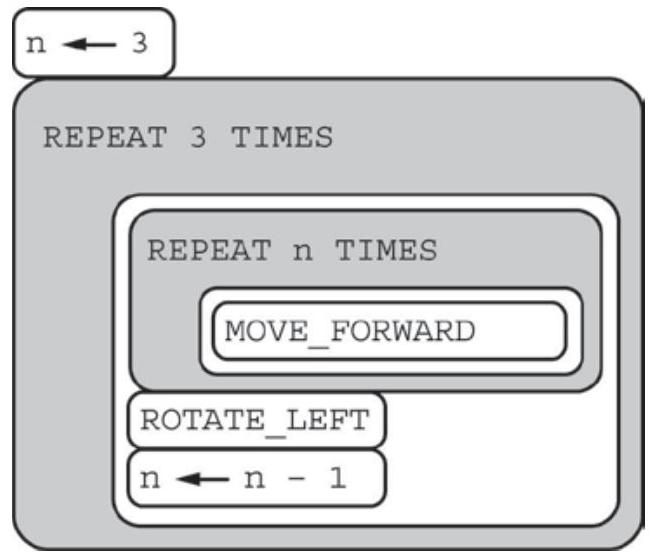
\includegraphics[max width=\textwidth, alt={}, center]{68b75e92-b243-4d72-a2a7-db8b0e1b4bf4-05_558_652_863_734}

Which of the following shows the location of the robot after running the code segment?

\begin{figure}[h]
\begin{center}
\captionsetup{labelformat=empty}
\caption{(A)}
  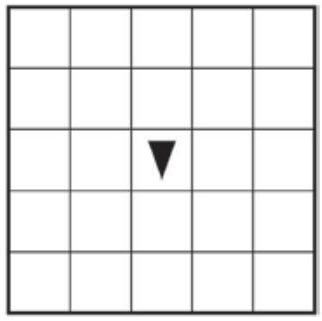
\includegraphics[alt={},max width=\textwidth]{68b75e92-b243-4d72-a2a7-db8b0e1b4bf4-05_321_322_1512_433}
\end{center}
\end{figure}

\begin{figure}[h]
\begin{center}
\captionsetup{labelformat=empty}
\caption{(B)}
  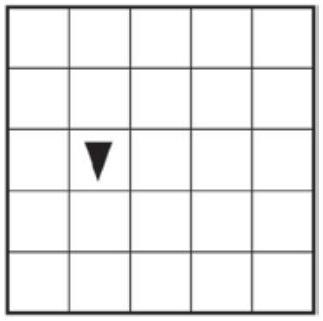
\includegraphics[alt={},max width=\textwidth]{68b75e92-b243-4d72-a2a7-db8b0e1b4bf4-05_321_323_1512_1194}
\end{center}
\end{figure}

\begin{figure}[h]
\begin{center}
\captionsetup{labelformat=empty}
\caption{(C)}
  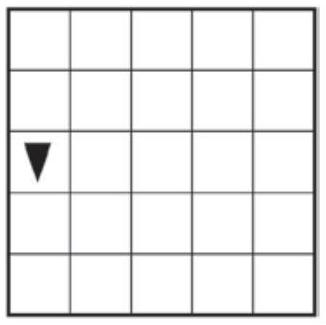
\includegraphics[alt={},max width=\textwidth]{68b75e92-b243-4d72-a2a7-db8b0e1b4bf4-05_325_326_1916_433}
\end{center}
\end{figure}

\begin{figure}[h]
\begin{center}
\captionsetup{labelformat=empty}
\caption{(D)}
  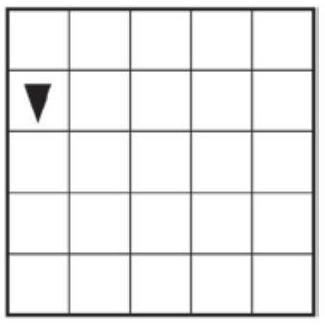
\includegraphics[alt={},max width=\textwidth]{68b75e92-b243-4d72-a2a7-db8b0e1b4bf4-05_325_325_1916_1194}
\end{center}
\end{figure}

\begin{center}
\begin{tabular}{|l|l|l|l|}
\hline
Enduring Understandings & Learning Objectives & Computational Thinking Practices & Essential Knowledge \\
\hline
5.2 People write programs to execute algorithms. & 5.2.1 Explain how programs implement algorithms. [P3] & P3 Abstracting & \begin{tabular}{l}
5.2.1A \\
5.2.1B \\
5.2.1C \\
\end{tabular} \\
\hline
\end{tabular}
\end{center}

\begin{enumerate}
  \setcounter{enumi}{5}
  \item Which of the following statements describes a limitation of using a computer simulation to model a real-world object or system?\\
(A) Computer simulations can only be built after the real-world object or system has been created.\\
(B) Computer simulations only run on very powerful computers that are not available to the general public.\\
(C) Computer simulations usually make some simplifying assumptions about the real-world object or system being modeled.\\
(D) It is difficult to change input parameters or conditions when using computer simulations.
\end{enumerate}

\begin{center}
\begin{tabular}{|l|l|l|l|}
\hline
Enduring Understandings & Learning Objectives & Computational Thinking Practices & Essential Knowledge \\
\hline
2.3 Models and simulations use abstraction to generate new understanding and knowledge. & 2.3.1 Use models and simulations to represent phenomena. [P3] & P3 Abstracting & \begin{tabular}{l}
2.3.1A \\
2.3.1C \\
2.3.1D \\
\end{tabular} \\
\hline
\end{tabular}
\end{center}

\begin{enumerate}
  \setcounter{enumi}{6}
  \item A certain social media Web site allows users to post messages and to comment on other messages that have been posted. When a user posts a message, the message itself is considered data. In addition to the data, the site stores the following metadata.
\end{enumerate}

\begin{itemize}
  \item The time the message was posted
  \item The name of the user who posted the message
  \item The names of any users who comment on the message and the times the comments were made
\end{itemize}

For which of the following goals would it be more useful to analyze the data instead of the metadata?\\
(A) To determine the users who post messages most frequently\\
(B) To determine the time of day that the site is most active\\
(C) To determine the topics that many users are posting about\\
(D) To determine which posts from a particular user have received the greatest number of comments

\begin{center}
\begin{tabular}{|l|l|l|l|}
\hline
Enduring Understandings & Learning Objectives & Computational Thinking Practices & Essential Knowledge \\
\hline
3.2 Computing facilitates exploration and the discovery of connections in information. & 3.2.1 Extract information from data to discover and explain connections or trends. [P1] & P1 Connecting computing & \begin{tabular}{l}
3.2.1B \\
3.2.1G \\
3.2.1H \\
3.2.1I \\
\end{tabular} \\
\hline
\end{tabular}
\end{center}

\begin{enumerate}
  \setcounter{enumi}{7}
  \item The program segment below is intended to move a robot in a grid to a gray square. The program segment uses the procedure GoalReached, which evaluates to true if the robot is in the gray square and evaluates to false otherwise. The robot in each grid is represented as a triangle and is initially facing left. The robot can move into a white or gray square but cannot move into a black region.
\end{enumerate}

\begin{verbatim}
REPEAT UNTIL (GoalReached ())
{
    IF (CAN_MOVE (forward))
    {
        MOVE_FORWARD ()
    }
    IF (CAN_MOVE (right))
    {
        ROTATE_RIGHT ()
    }
    IF (CAN_MOVE (left))
    {
        ROTATE_LEFT ()
    }
}
\end{verbatim}

For which of the following grids does the program NOT correctly move the robot to the gray square?\\
(A)\\
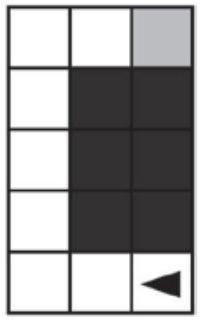
\includegraphics[max width=\textwidth, alt={}, center]{68b75e92-b243-4d72-a2a7-db8b0e1b4bf4-08_321_201_416_433}\\
(B)\\

\includegraphics[max width=\textwidth, alt={}, center]{68b75e92-b243-4d72-a2a7-db8b0e1b4bf4-08_321_201_416_1194}\\
(C)\\

\includegraphics[max width=\textwidth, alt={}, center]{68b75e92-b243-4d72-a2a7-db8b0e1b4bf4-08_321_201_820_433}\\
(D)\\

\includegraphics[max width=\textwidth, alt={}, center]{68b75e92-b243-4d72-a2a7-db8b0e1b4bf4-08_321_201_820_1194}

\begin{center}
\begin{tabular}{|l|l|l|l|}
\hline
Enduring Understandings & Learning Objectives & Computational Thinking Practices & Essential Knowledge \\
\hline
4.2 Algorithms can solve many, but not all, computational problems. & 4.2.4 Evaluate algorithms analytically and empirically for efficiency, correctness, and clarity. [P4] & P4 Analyzing problems and artifacts & 4.2.4B \\
\hline
\end{tabular}
\end{center}

\begin{enumerate}
  \setcounter{enumi}{8}
  \item The table below shows the time a computer system takes to complete a specified task on the customer data of different-sized companies.
\end{enumerate}

\begin{center}
\begin{tabular}{|l|l|l|l|}
\hline
Task & Small Company (approximately 100 customers) & Medium Company (approximately 1,000 customers) & Large Company (approximately 10,000 customers) \\
\hline
Backing up data & 2 hours & 20 hours & 200 hours \\
\hline
Deleting entries from data & 100 hours & 200 hours & 300 hours \\
\hline
Searching through data & 250 hours & 300 hours & 350 hours \\
\hline
Sorting data & 0.01 hour & 1 hour & 100 hours \\
\hline
\end{tabular}
\end{center}

Based on the information in the table, which of the following tasks is likely to take the longest amount of time when scaled up for a very large company of approximately 100,000 customers?\\
(A) Backing up data\\
(B) Deleting entries from data\\
(C) Searching through data\\
(D) Sorting data

\begin{center}
\begin{tabular}{|l|l|l|l|}
\hline
Enduring Understandings & Learning Objectives & Computational Thinking Practices & Essential Knowledge \\
\hline
3.2 Computing facilitates exploration and the discovery of connections in information. & 3.2.2 Determine how large data sets impact the use of computational processes to discover information and knowledge. [P3] & P3 Abstracting & \begin{tabular}{l}
3.2.2E \\
3.2.2F \\
3.2.2H \\
\end{tabular} \\
\hline
\end{tabular}
\end{center}

\begin{enumerate}
  \setcounter{enumi}{9}
  \item Consider the code segment below.\\
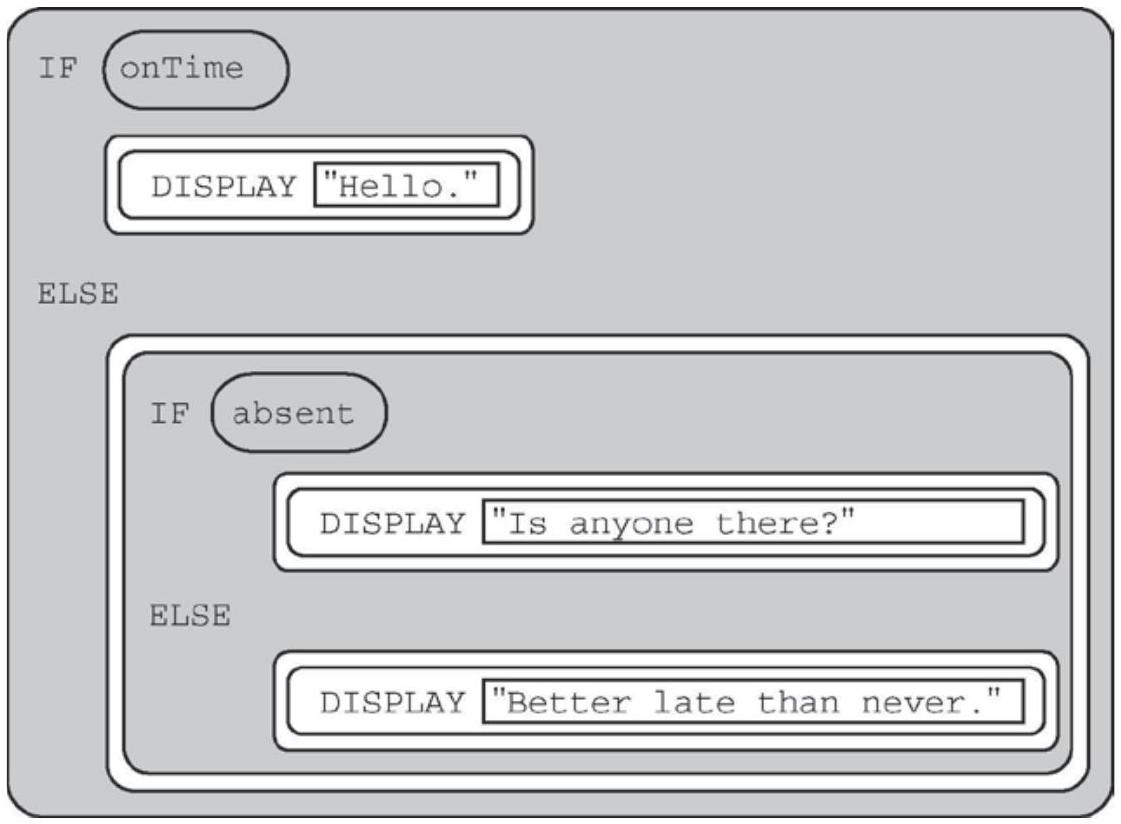
\includegraphics[max width=\textwidth, alt={}, center]{68b75e92-b243-4d72-a2a7-db8b0e1b4bf4-09_824_1121_1194_502}
\end{enumerate}

If the variables onTime and a.bsent both have the value false, what is displayed as a result of running the code segment?\\
(A) Is anyone there?\\
(B) Better late than never.\\
(C) Hello. Is anyone there?\\
(D) Hello. Better late than never.

\begin{center}
\begin{tabular}{|l|l|l|l|}
\hline
Enduring Understandings & Learning Objectives & Computational Thinking Practices & Essential Knowledge \\
\hline
4.1 Algorithms are precise sequences of instructions for processes that can be executed by a computer and are implemented using programming languages. & 4.1.1 Develop an algorithm for implementation in a program. [P2] & P2 Creating computational artifacts & \begin{tabular}{l}
4.1.1A \\
4.1.1C \\
\end{tabular} \\
\hline
\end{tabular}
\end{center}

\begin{enumerate}
  \setcounter{enumi}{10}
  \item Under which of the following conditions is it most beneficial to use a heuristic approach to solve a problem?\\
(A) When the problem can be solved in a reasonable time and an approximate solution is acceptable\\
(B) When the problem can be solved in a reasonable time and an exact solution is needed\\
(C) When the problem cannot be solved in a reasonable time and an approximate solution is acceptable\\
(D) When the problem cannot be solved in a reasonable time and an exact solution is needed
\end{enumerate}

\begin{center}
\begin{tabular}{|l|l|l|l|}
\hline
Enduring Understandings & Learning Objectives & Computational Thinking Practices & Essential Knowledge \\
\hline
4.2 Algorithms can solve many, but not all, computational problems. & 4.2.2 Explain the difference between solvable and unsolvable problems in computer science. [P1] & P1 Connecting computing & \begin{tabular}{l}
4.2.2A \\
4.2.2B \\
4.2.2C \\
\end{tabular} \\
\hline
\end{tabular}
\end{center}

\begin{enumerate}
  \setcounter{enumi}{11}
  \item Which of the following are true statements about digital certificates in Web browsers?\\
I. Digital certificates are used to verify the ownership of encrypted keys used in secured communication.\\
II. Digital certificates are used to verify that the connection to a Web site is fault tolerant.\\
(A) I only\\
(B) II only\\
(C) I and II\\
(D) Neither I nor II
\end{enumerate}

\begin{center}
\begin{tabular}{|l|l|l|l|}
\hline
Enduring Understandings & Learning Objectives & Computational Thinking Practices & Essential Knowledge \\
\hline
6.3 Cybersecurity is an important concern for the Internet and the systems built on it. & 6.3.1 Identify existing cybersecurity concerns and potential options that address these issues with the Internet and the systems built on it. [P1] & P1 Connecting computing & \begin{tabular}{l}
6.3.1H \\
6.3.1L \\
6.3.1M \\
\end{tabular} \\
\hline
\end{tabular}
\end{center}

\begin{enumerate}
  \setcounter{enumi}{12}
  \item There are 32 students standing in a classroom. Two different algorithms are given for finding the average height of the students.
\end{enumerate}

\section*{Algorithm A}
Step 1: All students stand.\\
Step 2: A randomly selected student writes his or her height on a card and is seated.\\
Step 3: A randomly selected standing student adds his or her height to the value on the card, records the new value on the card, and is seated. The previous value on the card is erased.

Step 4: Repeat step 3 until no students remain standing.\\
Step 5: The sum on the card is divided by 32 . The result is given to the teacher.

\section*{Algorithm B}
Step 1: All students stand.\\
Step 2: Each student is given a card. Each student writes his or her height on the card.\\
Step 3: Standing students form random pairs at the same time. Each pair adds the numbers written on their cards and writes the result on one student's card; the other student is seated. The previous value on the card is erased.

Step 4: Repeat step 3 until one student remains standing.\\
Step 5: The sum on the last student's card is divided by 32 . The result is given to the teacher.\\
Which of the following statements is true?\\
(A) Algorithm A always calculates the correct average, but Algorithm B does not.\\
(B) Algorithm B always calculates the correct average, but Algorithm A does not.\\
(C) Both Algorithm A and Algorithm B always calculate the correct average.\\
(D) Neither Algorithm A nor Algorithm B calculates the correct average.

\begin{center}
\begin{tabular}{|l|l|l|l|}
\hline
Enduring Understandings & Learning Objectives & Computational Thinking Practices & Essential Knowledge \\
\hline
4.2 Algorithms can solve many, but not all, computational problems. & 4.2.4 Evaluate algorithms analytically and empirically for efficiency, correctness, and clarity. [P4] & P4 Analyzing problems and artifacts & 4.2.4C \\
\hline
\end{tabular}
\end{center}

\begin{enumerate}
  \setcounter{enumi}{13}
  \item The figure below shows a robot in a grid of squares. The robot is represented as a triangle, which is initially facing upward. The robot can move into a white or gray square but cannot move into a black region.\\
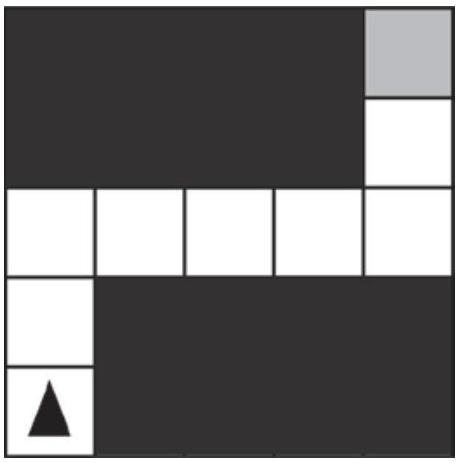
\includegraphics[max width=\textwidth, alt={}, center]{68b75e92-b243-4d72-a2a7-db8b0e1b4bf4-12_463_461_476_833}
\end{enumerate}

Consider the procedure MoveAndTurn below.

\begin{figure}[h]
\begin{center}
\captionsetup{labelformat=empty}
\caption{PROCEDURE MoveAndTurn numMoves, numTurns}
  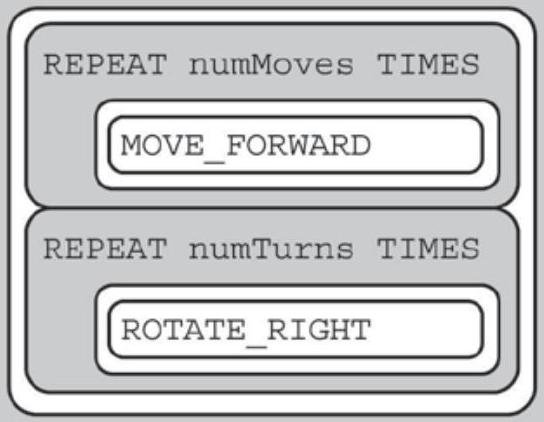
\includegraphics[alt={},max width=\textwidth]{68b75e92-b243-4d72-a2a7-db8b0e1b4bf4-12_422_544_1162_700}
\end{center}
\end{figure}

Which of the following code segments will move the robot to the gray square?

\begin{figure}[h]
\begin{center}
\captionsetup{labelformat=empty}
\caption{(A)}
  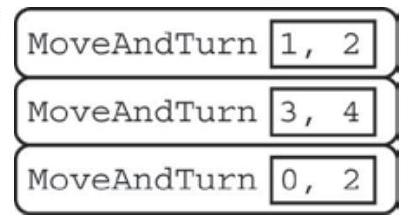
\includegraphics[alt={},max width=\textwidth]{68b75e92-b243-4d72-a2a7-db8b0e1b4bf4-12_222_409_1697_423}
\end{center}
\end{figure}

\begin{figure}[h]
\begin{center}
\captionsetup{labelformat=empty}
\caption{(B)}
  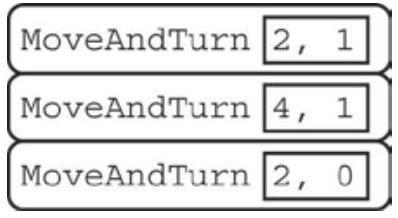
\includegraphics[alt={},max width=\textwidth]{68b75e92-b243-4d72-a2a7-db8b0e1b4bf4-12_218_398_1701_1190}
\end{center}
\end{figure}

\begin{figure}[h]
\begin{center}
\captionsetup{labelformat=empty}
\caption{(C)}
  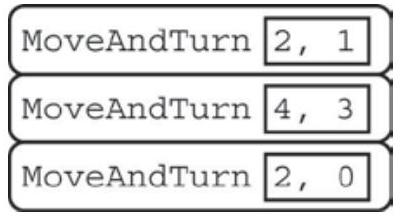
\includegraphics[alt={},max width=\textwidth]{68b75e92-b243-4d72-a2a7-db8b0e1b4bf4-12_218_403_2015_429}
\end{center}
\end{figure}

\begin{figure}[h]
\begin{center}
\captionsetup{labelformat=empty}
\caption{(D)}
  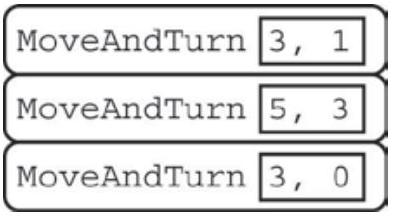
\includegraphics[alt={},max width=\textwidth]{68b75e92-b243-4d72-a2a7-db8b0e1b4bf4-12_218_394_2015_1194}
\end{center}
\end{figure}

\begin{center}
\begin{tabular}{|l|l|l|l|}
\hline
Enduring Understandings & Learning Objectives & Computational Thinking Practices & Essential Knowledge \\
\hline
5.3 Programming is facilitated by appropriate abstractions. & 5.3.1 Use abstraction to manage complexity in programs. [P3] & P3 Abstracting & \begin{tabular}{l}
5.3.1A \\
5.3.1B \\
5.3.1D \\
5.3.1E \\
5.3.1F \\
5.3.1G \\
\end{tabular} \\
\hline
\end{tabular}
\end{center}

\begin{enumerate}
  \setcounter{enumi}{14}
  \item Biologists often attach tracking collars to wild animals. For each animal, the following geolocation data is collected at frequent intervals.
\end{enumerate}

\begin{itemize}
  \item The time
  \item The date
  \item The location of the animal
\end{itemize}

Which of the following questions about a particular animal could NOT be answered using only the data collected from the tracking collars?\\
(A) Approximately how many miles did the animal travel in one week?\\
(B) Does the animal travel in groups with other tracked animals?\\
(C) Do the movement patterns of the animal vary according to the weather?\\
(D) In what geographic locations does the animal typically travel?

\begin{center}
\begin{tabular}{|l|l|l|l|}
\hline
Enduring Understandings & Learning Objectives & Computational Thinking Practices & Essential Knowledge \\
\hline
3.1 People use computer programs to process information to gain insight and knowledge. & 3.1.1 Find patterns and test hypotheses about digitally processed information to gain insight and knowledge. [P4] & P4 Analyzing problems and artifacts & 3.1.1E \\
\hline
\end{tabular}
\end{center}

\begin{enumerate}
  \setcounter{enumi}{15}
  \item A summer camp offers a morning session and an afternoon session. The list morningList contains the names of all children attending the morning session, and the list afternoonList contains the names of all children attending the afternoon session.
\end{enumerate}

Only children who attend both sessions eat lunch at the camp. The camp director wants to create lunchList, which will contain the names of children attending both sessions.

The following code segment is intended to create lunchList, which is initially empty. It uses the procedure IsFound (list, name), which returns true if name is found in list and returns false otherwise.

\begin{verbatim}
FOR EACH child IN morningList
{
    <MISSING CODE>
}
\end{verbatim}

Which of the following could replace<MISSING CODE> so that the code segment works as intended?

\begin{verbatim}
(A) IF (IsFound (afternoonList, child))
    {
        APPEND (lunchList, child)
    }
(B) IF (IsFound (lunchList, child))
    {
        APPEND (afternoonList, child)
    }
(C) IF (IsFound (morningList, child))
    {
        APPEND (lunchList, child)
    }
(D) IF ((IsFound (morningList, child)) OR
        (IsFound (afternoonList, child)))
    {
        APPEND (lunchList, child)
    }
\end{verbatim}

\begin{center}
\begin{tabular}{|l|l|l|l|}
\hline
Enduring Understandings & Learning Objectives & Computational Thinking Practices & Essential Knowledge \\
\hline
5.3 Programming is facilitated by appropriate abstractions. & 5.3.1 Use abstraction to manage complexity in programs. [P3] & P3 Abstracting & \begin{tabular}{l}
5.3.1G \\
5.3.1K \\
5.3.1L \\
\end{tabular} \\
\hline
\end{tabular}
\end{center}

\begin{enumerate}
  \setcounter{enumi}{16}
  \item Consider the following program code.\\
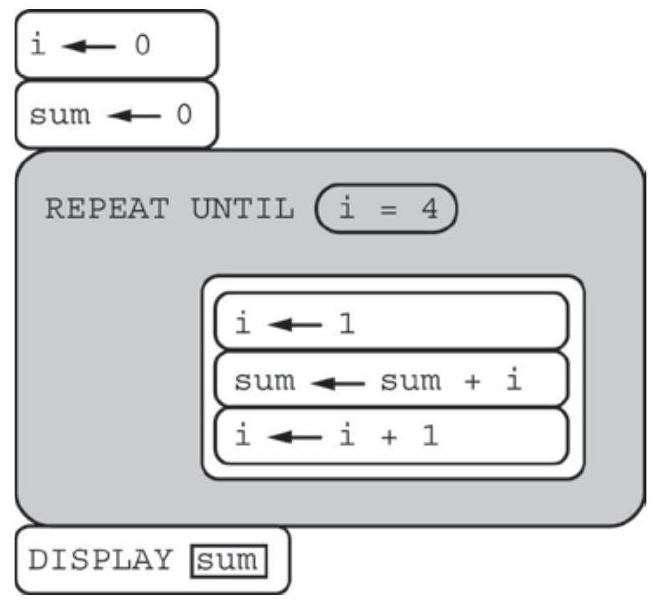
\includegraphics[max width=\textwidth, alt={}, center]{68b75e92-b243-4d72-a2a7-db8b0e1b4bf4-15_602_656_382_732}
\end{enumerate}

Which of the following best describes the result of running the program code?\\
(A) The number 0 is displayed.\\
(B) The number 6 is displayed.\\
(C) The number 10 is displayed.\\
(D) Nothing is displayed; the program results in an infinite loop.

\begin{center}
\begin{tabular}{|l|l|l|l|}
\hline
Enduring Understandings & Learning Objectives & Computational Thinking Practices & Essential Knowledge \\
\hline
5.4 Programs are developed, maintained, and used by people for different purposes. & 5.4.1 Evaluate the correctness of a program. [P4] & P4 Analyzing problems and artifacts & \begin{tabular}{l}
5.4.1E \\
5.4.1K \\
5.4.1N \\
\end{tabular} \\
\hline
\end{tabular}
\end{center}

\begin{enumerate}
  \setcounter{enumi}{17}
  \item Which of the following is a true statement about data compression?\\
(A) Data compression is only useful for files being transmitted over the Internet.\\
(B) Regardless of the compression technique used, once a data file is compressed, it cannot be restored to its original state.\\
(C) Sending a compressed version of a file ensures that the contents of the file cannot be intercepted by an unauthorized user.\\
(D) There are trade-offs involved in choosing a compression technique for storing and transmitting data.
\end{enumerate}

\begin{center}
\begin{tabular}{|l|l|l|l|}
\hline
Enduring Understandings & Learning Objectives & Computational Thinking Practices & Essential Knowledge \\
\hline
3.3 There are trade-offs when representing information as digital data. & 3.3.1 Analyze how data representation, storage, security, and transmission of data involve computational manipulation of information. [P4] & P4 Analyzing problems and artifacts & \begin{tabular}{l}
3.3.1C \\
3.3.1D \\
3.3.1E \\
\end{tabular} \\
\hline
\end{tabular}
\end{center}

\begin{enumerate}
  \setcounter{enumi}{18}
  \item An office building has two floors. A computer program is used to control an elevator that travels between the two floors. Physical sensors are used to set the following Boolean variables.
\end{enumerate}

\begin{center}
\begin{tabular}{|l|l|}
\hline
Variable & Description \\
\hline
onFloor1 & set to true if the elevator is stopped on floor 1; otherwise set to false \\
\hline
onFloor2 & set to true if the elevator is stopped on floor 2; otherwise set to false \\
\hline
callTo1 & set to true if the elevator is called to floor 1; otherwise set to false \\
\hline
callTo2 & set to true if the elevator is called to floor 2; otherwise set to false \\
\hline
\end{tabular}
\end{center}

The elevator moves when the door is closed and the elevator is called to the floor that it is not currently on. Which of the following Boolean expressions can be used in a selection statement to cause the elevator to move?\\
(A) (onFloor1 AND callTo2) AND (onFloor2 AND callTo1)\\
(B) (onFloor1 AND callTo2) OR (onFloor2 AND callTo1)\\
(C) (onFloor1 OR callTo2) AND (onFloor2 OR callTo1)\\
(D) (onFloor1 OR callTo2) OR (onFloor2 OR callTo1)

\begin{center}
\begin{tabular}{|l|l|l|l|}
\hline
Enduring Understandings & Learning Objectives & Computational Thinking Practices & Essential Knowledge \\
\hline
5.5 Programming uses mathematical and logical concepts. & 5.5.1 Employ appropriate mathematical and logical concepts in programming. [P4] & P1 Connecting computing & \begin{tabular}{l}
5.5.1E \\
5.5.1F \\
5.5.1G \\
\end{tabular} \\
\hline
\end{tabular}
\end{center}

\begin{enumerate}
  \setcounter{enumi}{19}
  \item According to the domain name system (DNS), which of the following is a subdomain of the domain \href{http://example.com}{example.com}?\\
(A) \href{http://about.example.com}{about.example.com}\\
(B) \href{http://example.co.uk}{example.co.uk}\\
(C) \href{http://example.com.org}{example.com.org}\\
(D) \href{http://example.org}{example.org}
\end{enumerate}

\begin{center}
\begin{tabular}{|l|l|l|l|}
\hline
Enduring Understandings & Learning Objectives & Computational Thinking Practices & Essential Knowledge \\
\hline
6.2 Characteristics of the Internet influence the systems built on it. & 6.2.1 Explain characteristics of the Internet and the systems built on it. [P5] & P5 Communicating & 6.2.1B \\
\hline
\end{tabular}
\end{center}

\begin{enumerate}
  \setcounter{enumi}{20}
  \item Which of the following algorithms require both selection and iteration?
\end{enumerate}

Select two answers.\\
(A) An algorithm that, given two integers, displays the greater of the two integers\\
(B) An algorithm that, given a list of integers, displays the number of even integers in the list\\
(C) An algorithm that, given a list of integers, displays only the negative integers in the list\\
(D) An algorithm that, given a list of integers, displays the sum of the integers in the list

\begin{center}
\begin{tabular}{|l|l|l|l|}
\hline
Enduring Understandings & Learning Objectives & Computational Thinking Practices & Essential Knowledge \\
\hline
4.1 Algorithms are precise sequences of instructions for processes that can be executed by a computer and are implemented using programming languages. & 4.1.1 Develop an algorithm for implementation in a program. [P2] & P2 Creating computational artifacts & \begin{tabular}{l}
4.1.1A \\
4.1.1C \\
4.1.1D \\
\end{tabular} \\
\hline
\end{tabular}
\end{center}

\begin{enumerate}
  \setcounter{enumi}{21}
  \item A teacher uses the following program to adjust student grades on an assignment by adding 5 points to each student's original grade. However, if adding 5 points to a student's original grade causes the grade to exceed 100 points, the student will receive the maximum possible score of 100 points. The students' original grades are stored in the list gradeList, which is indexed from 1 to n .
\end{enumerate}

\begin{verbatim}
i \leftarrow 1
REPEAT n TIMES
{
    <MISSING CODE>
    i \leftarrow i + 1
}
\end{verbatim}

The teacher has the following procedures available.

\begin{center}
\begin{tabular}{|l|l|}
\hline
Procedure & Explanation \\
\hline
$\min (\mathrm{a}, \mathrm{b})$ & Returns the lesser of the two values a and b \\
\hline
$\max (\mathrm{a}, \mathrm{b})$ & Returns the greater of the two values a and b \\
\hline
\end{tabular}
\end{center}

Which of the following code segments can replace<MISSING CODE> so that the program works as intended?

Select two answers.

\begin{verbatim}
(A) gradeList[i] ← min (gradeList[i] + 5, 100)
(B) gradeList[i] ← max (gradeList[i] + 5, 100)
(C) gradeList[i] ← gradeList[i] + 5
    IF (gradeList[i]> 100)
    {
    gradeList[i] ← gradeList[i] - 5
    }
(D) gradeList[i] ← gradeList[i] + 5
    IF (gradeList[i] > 100)
    {
    gradeList[i]←100
    }
\end{verbatim}

\begin{center}
\begin{tabular}{|l|l|l|l|}
\hline
Enduring Understandings & Learning Objectives & Computational Thinking Practices & Essential Knowledge \\
\hline
5.5 Programming uses mathematical and logical concepts. & 5.5.1 Employ appropriate mathematical and logical concepts in programming. [P1] & P1 Connecting computing & \begin{tabular}{l}
5.5.1A \\
5.5 .1 B \\
5.5.1H \\
\end{tabular} \\
\hline
\end{tabular}
\end{center}

\section*{Answers to Sample Exam Questions}
\begin{center}
\begin{tabular}{|l|l|}
\hline
1 - C & 12 - A \\
\hline
2 - C & 13 - C \\
\hline
3 - C & 14 - C \\
\hline
4 - A & 15 - C \\
\hline
$5-\mathrm{A}$ & 16 - A \\
\hline
6 - C & 17 - D \\
\hline
7 - C & 18 - D \\
\hline
8 - D & 19 - B \\
\hline
9 - D & 20 - A \\
\hline
10 - B & 21 - B, C \\
\hline
11 - C & 22 - A, D \\
\hline
\end{tabular}
\end{center}


\end{document}